\chapter{रासायनिक स्पीशीज़, प्राकृतिक और संश्लिष्ट}\label{ch:g10:chemical-species}

वनीला आइसक्रीम की एक चम्मच। उसका स्वाद एक उष्णकटिबंधीय ऑर्किड की काली फलियों
से आ सकता है, जिन्हें तोड़ा, पकाया और महीनों ऐल्कोहॉल में भिगोया गया हो; या वह
ऐसे कारख़ाने से आ सकता है जो यह स्वाद लकड़ी की लुगदी या तेल से बनाता है। दोनों
को साथ-साथ चखिए, तो मुख्य स्वाद एक ही है --- और इसका एक ठोस कारण है: जिस \omterm{def:g7:atoms-and-molecules:molecule}{अणु}
का स्वाद वनीला जैसा है, वैनिलिन, वह ठीक वही \omterm{def:g7:atoms-and-molecules:molecule}{अणु} है, चाहे वह किसी भी रास्ते से
मिला हो। यह अध्याय दिखाता है कि रसायनज्ञ किसी पौधे से कोई स्पीशीज़ कैसे निकालते
हैं, उसे कैसे बनाते हैं, और यह कैसे जाँचते हैं कि उनके पास जो है वह वही है जो
वे सोचते हैं।

\begin{recall}
\omterm{def:g6:pure-substances-and-mixtures:species}{रासायनिक स्पीशीज़} किसी पदार्थ का एक विशेष प्रकार है; \omterm{def:g6:pure-substances-and-mixtures:pure-substance}{शुद्ध पदार्थ} में एक स्पीशीज़
होती है और उसके निश्चित स्थिरांक होते हैं, जैसे उसके गलन और क्वथन ताप
(\cref{ch:g6:pure-substances-and-mixtures})। द्रव \omterm{def:g6:solutions-and-solubility:miscible}{मिश्रणीय} या \omterm{def:g6:solutions-and-solubility:miscible}{अमिश्रणीय} होते
हैं, और हर \omterm{def:g6:solutions-and-solubility:solute}{विलेय} की हर \omterm{def:g6:solutions-and-solubility:solute}{विलायक} में अपनी \omterm{def:g6:solutions-and-solubility:solubility}{विलेयता} होती है
(\cref{ch:g6:solutions-and-solubility})। \omterm{def:g7:identifying-substances:chromatography}{पेपर वर्णलेखन} किसी \omterm{def:g6:pure-substances-and-mixtures:mixture}{मिश्रण} के रंजकों
को अलग करता है
(\cref{ch:g7:identifying-substances})।
\end{recall}

\begin{omfigure}
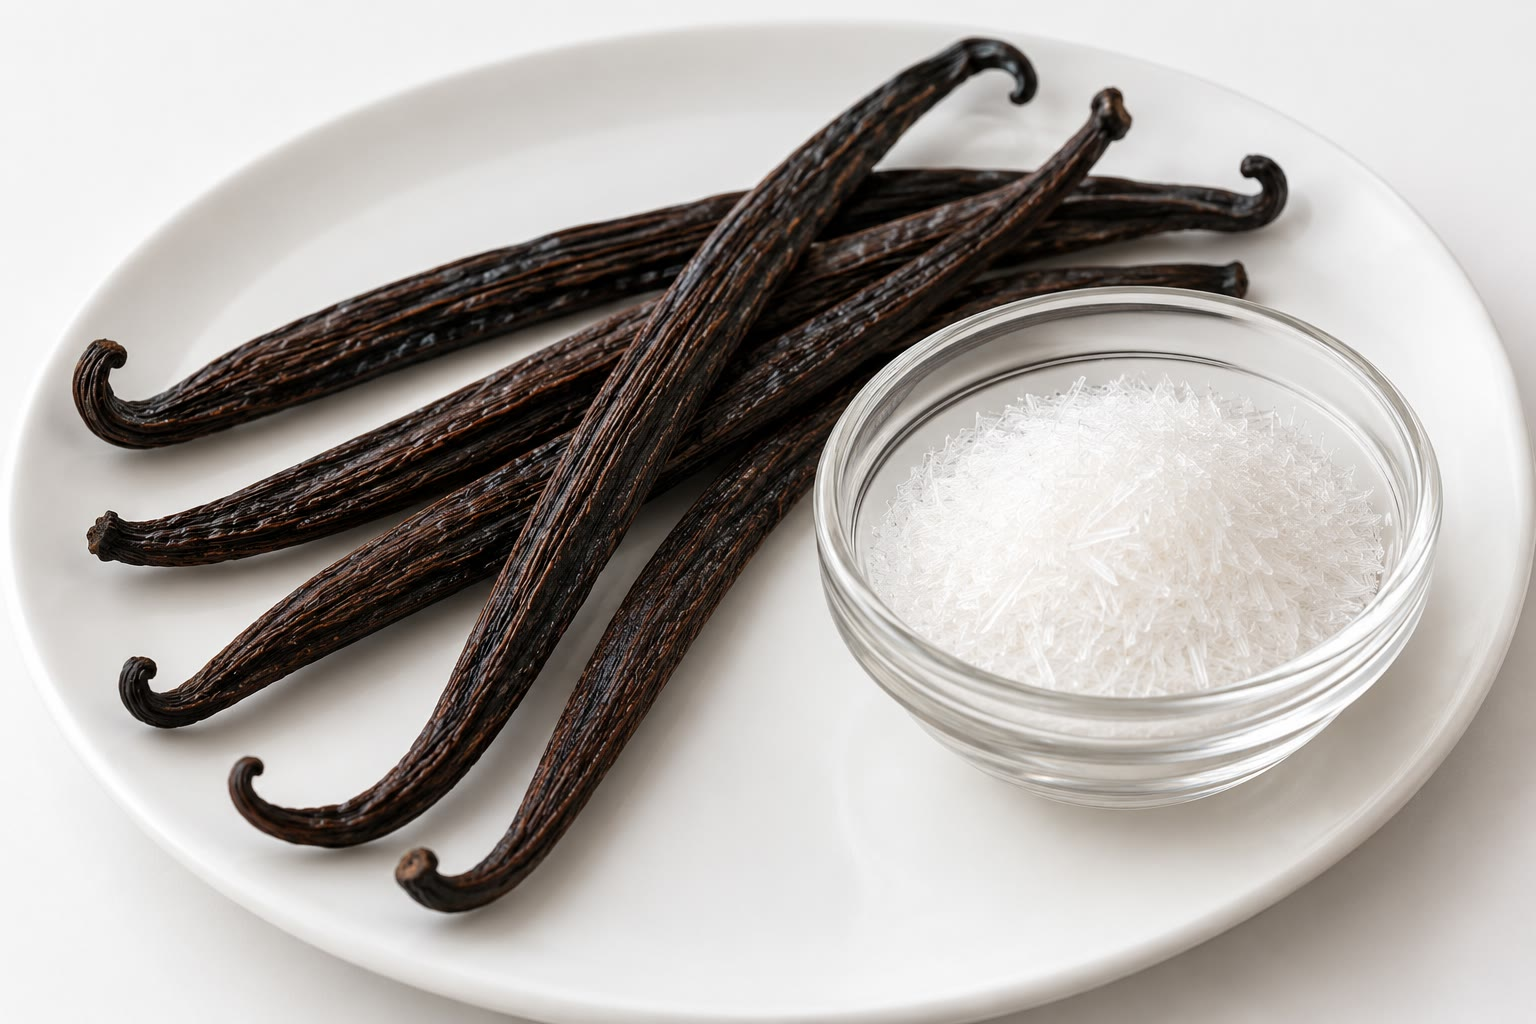
\includegraphics[width=0.55\linewidth]{images/book1/ai/g10-vanilla.jpg}

{\small वनीला की फलियाँ और वैनिलिन के सफ़ेद क्रिस्टल: एक ही \omterm{def:g7:atoms-and-molecules:molecule}{अणु},
पौधे से या कारख़ाने से।}
\end{omfigure}

\section{प्राकृतिक और संश्लिष्ट स्पीशीज़}

\begin{definition}[प्राकृतिक और संश्लिष्ट स्पीशीज़]\label{def:g10:chemical-species:natural}
\emph{प्राकृतिक स्पीशीज़}\index{प्राकृतिक स्पीशीज़} वह \omterm{def:g6:pure-substances-and-mixtures:species}{रासायनिक स्पीशीज़} है
जो किसी सजीव द्वारा बनाई जाती है या प्रकृति में उसी रूप में मिलती है। \emph{संश्लिष्ट
स्पीशीज़}\index{संश्लिष्ट स्पीशीज़} रसायनज्ञ दूसरी स्पीशीज़ से \omterm{def:g7:chemical-reactions:reaction}{रासायनिक
अभिक्रियाओं} द्वारा बनाते हैं। कोई संश्लिष्ट स्पीशीज़ किसी प्राकृतिक स्पीशीज़ जैसी
ही हो सकती है (संश्लिष्ट वैनिलिन), या प्रकृति में उसका कोई समकक्ष न हो (ज़्यादातर
दवाइयाँ और \omterm{def:g8:plastics:plastic}{प्लास्टिक})।
\end{definition}

\begin{proposition}[एक ही स्पीशीज़, एक ही गुण]\label{prop:g10:chemical-species:same}
किसी \omterm{def:g6:pure-substances-and-mixtures:species}{रासायनिक स्पीशीज़} के गुण उसके स्रोत से स्वतंत्र होते हैं:
कारख़ाने में बना वैनिलिन और फली से निकाला गया वैनिलिन, दोनों का सूत्र, गलनांक
और गंध एक ही है। जो अलग हो सकता है, वह है जो उसके साथ आता है: प्राकृतिक सत्
एक \omterm{def:g6:pure-substances-and-mixtures:mixture}{मिश्रण} है, जिसमें बहुत-सी दूसरी स्पीशीज़ होती हैं जो उसका स्वाद
बदलती हैं।
\end{proposition}

\begin{history}[विलो की छाल से ऐस्पिरिन तक, 1828--1899]
सदियों तक बुख़ार और दर्द के लिए विलो की छाल चबाई जाती रही। 1828 में एक
रसायनज्ञ ने उससे सक्रिय स्पीशीज़, सैलिसिन, निकाली; फिर रसायनज्ञों ने उसे
सैलिसिलिक अम्ल में बदला, जो असर करता है पर पेट में जलन करता है। 1897 में
रंजक और दवा बनाने वाली एक कंपनी में फ़ेलिक्स हॉफ़मान ने सैलिसिलिक अम्ल से एक
कोमल \omterm{def:g10:chemical-species:natural}{संश्लिष्ट स्पीशीज़} बनाई: ऐसीटिलसैलिसिलिक अम्ल, जो 1899 से ऐस्पिरिन के नाम से
बिका। ऐस्पिरिन का कोई प्राकृतिक स्रोत नहीं है: यह पूरी तरह \omterm{def:g10:chemical-species:natural}{संश्लिष्ट स्पीशीज़} है।
\end{history}

\section{किसी स्पीशीज़ का निष्कर्षण}

\begin{definition}[निष्कर्षण और द्रव--द्रव निष्कर्षण]\label{def:g10:chemical-species:extraction}
\emph{निष्कर्षण}\index{निष्कर्षण} किसी \omterm{def:g6:pure-substances-and-mixtures:species}{रासायनिक स्पीशीज़} को उस सामग्री से बाहर
निकालता है जिसमें वह है, आम तौर पर उसे किसी सोच-समझकर चुने गए \omterm{def:g6:solutions-and-solubility:solute}{विलायक} में घोलकर।
\emph{द्रव--द्रव निष्कर्षण}\index{द्रव--द्रव निष्कर्षण} में
एक द्रव में घुली स्पीशीज़ को ऐसे दूसरे द्रव में ले जाया जाता है जो पहले के साथ
\omterm{def:g6:solutions-and-solubility:miscible}{अमिश्रणीय} हो और जिसमें वह बेहतर \omterm{def:g2:mixing-and-dissolving:dissolve}{घुलती} हो;
फिर दोनों द्रवों को पृथक्कारी कीप में अलग किया जाता है।
\end{definition}

\begin{example}[रोज़मर्रा के निष्कर्षण]\label{ex:g10:chemical-species:everyday}
चाय बनाना गरम पानी से किया गया \omterm{def:g10:chemical-species:extraction}{निष्कर्षण} है (अर्क); वनीला की फलियों को ऐल्कोहॉल
में भिगोना एथेनॉल से किया गया \omterm{def:g10:chemical-species:extraction}{निष्कर्षण} है (मैसरेशन); शोरबा बनाने के लिए सब्ज़ियाँ
उबालना एक और \omterm{def:g10:chemical-species:extraction}{निष्कर्षण} है (काढ़ा)।
\end{example}


\begin{definition}[आसवन और जल-आसवन]\label{def:g10:chemical-species:distillation}
\emph{आसवन}\index{आसवन} किसी द्रव \omterm{def:g6:pure-substances-and-mixtures:mixture}{मिश्रण} को उबलने तक गरम करता है, बहते पानी
से ठंडे किए गए संघनित्र में वाष्प को फिर द्रव में बदलता है, और इस द्रव, यानी
आसुत, को इकट्ठा करता है।
\emph{जल-आसवन}\index{जल-आसवन} किसी पादप सामग्री को
पानी में उबालता है: भाप पौधे की सुगंधित स्पीशीज़ को साथ ले जाती है, जो आसुत में
पानी से अलग होकर एक तैलीय परत बनाती हैं: यही
सगंध तेल है।
\end{definition}

\begin{omfigure}
\begin{tikzpicture}[font=\small, scale=0.95]
  \pic[transform shape] at (0,0) {heatingmantle};
  \pic[transform shape] at (0,0) {rbflask={0.55}{omWater!70}};
  \foreach \x/\y in {-0.45/0.35,-0.1/0.55,0.3/0.3,0.5/0.7,-0.6/0.75,0.1/0.9,-0.25/0.2}
    \fill[green!45!black!70] (\x,\y) ellipse (0.09 and 0.04);
  \pic[transform shape] (s) at (0,3.0) {stillhead};
  \pic[transform shape] at ($(s-top)+(0,-0.75)$) {thermometer};
  \pic[transform shape, rotate=-20] (c) at (s-arm) {liebig={3.2}};
  \coordinate (cend) at ($(s-arm)+(-20:3.2)$);
  \pic[transform shape] (a) at (cend) {adapter};
  \pic[transform shape] at ($(a-tip)+(0,-2.3)$) {erlenmeyer={0.18}{omWater!70}};
  \fill[yellow!60!orange!60] ($(a-tip)+(-0.827,-2.3+0.47)$) -- ($(a-tip)+(0.827,-2.3+0.47)$) -- ($(a-tip)+(0.779,-2.3+0.6)$) -- ($(a-tip)+(-0.779,-2.3+0.6)$) -- cycle;
  \draw[<-, omProp, thick] (-0.55,0.55) -- (-2.2,0.9) node[left, text=black, align=right]
    {पानी और\\ लैवेंडर के फूल};
  \draw[<-, omProp, thick] (1.35,-0.6) -- (2.2,-1.1) node[right, text=black]
    {तापन मैंटल};
  \draw[<-, omProp, thick] (0.1,4.2) -- (-1.2,4.6) node[left, text=black] {तापमापी};
  \draw[<-, omProp, thick] ($(s-arm)+(-20:1.6)+(0,0.32)$) -- ++(0.6,1.0) node[above, text=black]
    {संघनित्र, बहते पानी से ठंडा};
  \draw[<-, omProp, thick] ($(a-tip)+(0.4,-1.88)$) -- ++(1.1,0.2) node[right, text=black, align=left]
    {आसुत: पानी पर तैरता\\ सगंध तेल};
\end{tikzpicture}

{\small लैवेंडर का \omterm{def:g10:chemical-species:distillation}{जल-आसवन}। भाप सगंध तेल को संघनित्र में ले जाती है;
आसुत अलग होकर पानी के ऊपर तेल की एक पतली परत
बनाता है।}
\end{omfigure}

\begin{method}[निष्कर्षण विलायक चुनना]\label{met:g10:chemical-species:solvent}
पानी से किसी स्पीशीज़ के \omterm{def:g10:chemical-species:extraction}{द्रव--द्रव निष्कर्षण} के लिए \omterm{def:g6:solutions-and-solubility:solute}{विलायक} को
चाहिए कि वह:
\begin{enumerate}
  \item स्पीशीज़ को पानी से कहीं बेहतर घोले;
  \item पानी के साथ \omterm{def:g6:solutions-and-solubility:miscible}{अमिश्रणीय} हो, ताकि दो परतें बनें;
  \item जितना संभव हो कम ख़तरनाक हो, और बाद में आसानी से हटाया जा सके
        (कम क्वथन ताप उसे वाष्पित होने देता है)।
\end{enumerate}
कौन-सी परत ऊपर होगी, यह घनत्व तय करते हैं: कम घना द्रव
तैरता है।
\end{method}

\begin{example}[लैवेंडर तेल के लिए विलायक]\label{ex:g10:chemical-species:table}
% ledger: rho:cyclohexane, bp:cyclohexane, rho:ethyl-acetate, bp:ethyl-acetate, rho:CH2Cl2, bp:CH2Cl2, rho:ethanol, bp:ethanol, sol:linalool
लिनालूल, लैवेंडर तेल की मुख्य स्पीशीज़, पानी में केवल
\qty{1.6}{g/L} तक \omterm{def:g2:mixing-and-dissolving:dissolve}{घुलता} है, पर नीचे दिए \omterm{def:g6:solutions-and-solubility:solute}{विलायकों} में बहुत अच्छी तरह:
\begin{center}
\small
\begin{tabular}{lccll}
\hline
\omterm{def:g6:solutions-and-solubility:solute}{विलायक} & \qty{1}{mL} का द्रव्यमान & उबलता है & पानी के साथ & मुख्य ख़तरे \\
\hline
साइक्लोहेक्सेन & \qty{0.78}{g} & \qty{81}{\celsius} & \omterm{def:g6:solutions-and-solubility:miscible}{अमिश्रणीय} & ज्वलनशील, हानिकारक \\
एथिल एथेनोएट & \qty{0.90}{g} & \qty{77}{\celsius} & \omterm{def:g6:solutions-and-solubility:miscible}{अमिश्रणीय} & ज्वलनशील, उत्तेजक \\
डाइक्लोरोमेथेन & \qty{1.33}{g} & \qty{40}{\celsius} & \omterm{def:g6:solutions-and-solubility:miscible}{अमिश्रणीय} & संदिग्ध कैंसरजन \\
एथेनॉल & \qty{0.79}{g} & \qty{78}{\celsius} & \omterm{def:g6:solutions-and-solubility:miscible}{मिश्रणीय} & ज्वलनशील \\
\hline
\end{tabular}
\end{center}
एथेनॉल का उपयोग नहीं हो सकता: वह पानी में मिल जाता है और कोई परत नहीं बनती।
साइक्लोहेक्सेन या एथिल एथेनोएट के साथ \omterm{def:g6:solutions-and-solubility:solute}{विलायक} की परत ऊपर होती है;
डाइक्लोरोमेथेन के साथ नीचे।
\end{example}

\begin{omfigure}
\begin{tikzpicture}[font=\small, scale=1.2]
  \pic[transform shape] at (0,0) {sepfunnel={omWater!70}{yellow!35!orange!35}};
  \draw[<-, omProp, thick] (0.55,2.1) -- (1.6,2.4) node[right, text=black, align=left]
    {साइक्लोहेक्सेन और तेल\\ (कम घना, ऊपर)};
  \draw[<-, omProp, thick] (0.55,1.3) -- (1.6,1.2) node[right, text=black, align=left]
    {पानी, टोंटी से\\ निकाला जाता है};
  \draw[<-, omProp, thick] (0.25,0.52) -- (1.6,0.4) node[right, text=black] {टोंटी};
\end{tikzpicture}

{\small हिलाने और ठहरने के बाद पृथक्कारी कीप: तेल ऊपर वाले साइक्लोहेक्सेन
में चला गया है।}
\end{omfigure}

\begin{safety}{\ghs[0.8cm]{GHS02}\ghs[0.8cm]{GHS07}\ghs[0.8cm]{GHS08}\ghs[0.8cm]{GHS09}}
% ledger: ghs:cyclohexane
साइक्लोहेक्सेन: अत्यधिक ज्वलनशील (GHS02); निगलने पर और श्वासनली में जाने पर
घातक हो सकता है, त्वचा में जलन और उनींदापन करता है (GHS07, GHS08);
जलीय जीवों के लिए अत्यंत विषैला (GHS09)। इसे धूम-हुड के नीचे, लौ से दूर,
इस्तेमाल किया जाता है।
\end{safety}

\section{पतली परत वर्णलेखन}

\begin{definition}[पतली परत वर्णलेखन]\label{def:g10:chemical-species:tlc}
\emph{पतली परत वर्णलेखन}\index{पतली परत वर्णलेखन} (TLC)
किसी \omterm{def:g6:pure-substances-and-mixtures:mixture}{मिश्रण} की स्पीशीज़ को ऐसी प्लेट पर अलग करता है जिस पर एक बारीक सफ़ेद चूर्ण
की पतली परत चढ़ी होती है; यह परत \emph{स्थिर प्रावस्था}\index{स्थिर प्रावस्था} है।
नमूनों के छोटे धब्बे नीचे के पास पेंसिल की एक रेखा पर लगाए जाते हैं; प्लेट एक बंद
टंकी में थोड़े-से \omterm{def:g6:solutions-and-solubility:solute}{विलायक} में खड़ी की जाती है, जिसे
\emph{निक्षालक}\index{निक्षालक} कहते हैं; वह प्लेट पर चढ़ता है और हर
स्पीशीज़ को उस ऊँचाई तक ले जाता है जो स्पीशीज़ पर निर्भर करती है। फिर रंगहीन
धब्बों को पराबैंगनी प्रकाश में या आयोडीन वाष्प से प्रकट किया जाता है।
\end{definition}

\begin{definition}[मंदन गुणांक]\label{def:g10:chemical-species:retention-factor}
किसी धब्बे का \emph{मंदन गुणांक}\index{मंदन गुणांक} है
\[
  R_f = \frac{\text{प्रारंभ-रेखा से धब्बे तक की दूरी}}
             {\text{प्रारंभ-रेखा से विलायक अग्र तक की दूरी}},
\]
जो 0 और 1 के बीच की एक संख्या है। दी गई प्लेट, \omterm{def:g10:chemical-species:tlc}{निक्षालक} और ताप के लिए
हर स्पीशीज़ का अपना $R_f$ होता है।
\end{definition}

\begin{method}[TLC करना और पढ़ना]\label{met:g10:chemical-species:tlc}
\begin{enumerate}
  \item नीचे से \qty{1}{cm} पर पेंसिल से प्रारंभ-रेखा खींचिए;
        उस पर हर नमूने का और हर संदर्भ स्पीशीज़ का एक छोटा धब्बा
        लगाइए।
  \item प्लेट को टंकी में खड़ा कीजिए, \omterm{def:g10:chemical-species:tlc}{निक्षालक} रेखा से नीचे रहे; टंकी
        बंद कीजिए।
  \item जब अग्र ऊपर से लगभग \qty{1}{cm} दूर रह जाए, तो प्लेट निकालिए;
        तुरंत अग्र पर निशान लगाइए; सुखाइए और धब्बे प्रकट कीजिए।
  \item दूरियाँ मापिए और हर धब्बे का $R_f$ निकालिए। एक धब्बा देने वाला
        नमूना शायद एक शुद्ध स्पीशीज़ है; उसी प्लेट पर किसी संदर्भ धब्बे जितनी
        ऊँचाई वाला धब्बा शायद वही
        स्पीशीज़ है।
\end{enumerate}
\end{method}

\begin{omfigure}
\begin{tikzpicture}[font=\small, scale=1.25]
  % the tank
  \pic[transform shape] at (0,0) {beaker={0.15}{omWater!80}};
  \fill[white] (-0.55,0.08) rectangle (0.55,1.92);
  \fill[omWater!80] (-0.55,0.08) rectangle (0.55,0.3);
  \draw[omGlass, line width=0.6pt] (-0.55,0.08) rectangle (0.55,1.92);
  \draw[black!60] (-0.55,0.42) -- (0.55,0.42);
  \foreach \x in {-0.3,0,0.3} \fill[black!70] (\x,0.42) circle (0.04);
  \fill[black!25] (-1.0,2.08) rectangle (1.0,2.18);
  \node[anchor=north, align=center] at (0,-0.15) {ढक्कन से बंद\\ टंकी};
  % the developed plate
  \begin{scope}[xshift=4.2cm]
    \pic[transform shape] at (0,0) {tlcplate};
    \draw[black!50, dashed] (-0.7,2.8) -- (0.7,2.8);
    \fill[omDef!70] (-0.35,1.36) ellipse (0.1 and 0.07);
    \fill[omDef!70] (-0.35,2.2) ellipse (0.1 and 0.07);
    \fill[omDef!70] (0,1.36) ellipse (0.1 and 0.07);
    \fill[omDef!70] (0.35,2.2) ellipse (0.1 and 0.07);
    \foreach \x/\l in {-0.35/O,0/L,0.35/A} \node[font=\footnotesize, anchor=north] at (\x,0.38) {\l};
    \draw[<->, omProp] (0.95,0.4) -- (0.95,1.36) node[midway, right, text=black, font=\footnotesize] {$d$};
    \draw[<->, omProp] (1.55,0.4) -- (1.55,2.8) node[midway, right, text=black, font=\footnotesize] {$D$};
    \draw[black!40, densely dotted] (-0.25,1.36) -- (0.95,1.36);
    \node[anchor=north, align=center] at (0.2,-0.15) {विकसित प्लेट:\\ $R_f = d/D$};
  \end{scope}
\end{tikzpicture}

{\small लिनालूल (L) और लिनालिल एथेनोएट (A) के बगल में लैवेंडर तेल (O) का
TLC। तेल दो धब्बे देता है, दोनों संदर्भों की ऊँचाइयों पर: उसमें दोनों स्पीशीज़
हैं। लिनालूल के लिए $R_f = d/D$।}
\end{omfigure}

\section{भौतिक स्थिरांकों से स्पीशीज़ की पहचान}

\begin{proposition}[गलनांक पहचान और शुद्धता की जाँच करता है]\label{prop:g10:chemical-species:mp}
% ledger: mp:vanillin, mp:aspirin, mp:salicylic
शुद्ध ठोस अपने ताप पर तीक्ष्णता से पिघलता है: वैनिलिन लगभग
\qty{82}{\celsius} पर, ऐस्पिरिन \qty{135}{\celsius} पर, सैलिसिलिक अम्ल
\qty{158}{\celsius} पर। अशुद्ध नमूना कम ताप पर, और कई डिग्री के परास में
पिघलता है। इसलिए गरम धातु-पट्टी पर या गलनांक उपकरण में गलनांक मापना
किसी ठोस को पहचानता भी है और यह भी बताता है कि वह
शुद्ध है या नहीं।
\end{proposition}

\begin{inthelab}[एक TLC प्लेट]
छात्र एक प्लेट पर लैवेंडर तेल, लिनालूल और लिनालिल एथेनोएट के धब्बे लगाते हैं,
उसे शिक्षक द्वारा चुने गए \omterm{def:g6:solutions-and-solubility:solute}{विलायकों} के \omterm{def:g6:pure-substances-and-mixtures:mixture}{मिश्रण} वाले बंद जार में विकसित करते हैं,
और पराबैंगनी रोकने वाला चश्मा पहनकर पराबैंगनी लैंप के नीचे धब्बे प्रकट करते हैं।
\omterm{def:g10:chemical-species:tlc}{निक्षालक} का उपयोग और रख-रखाव धूम-हुड के नीचे
होता है।
\end{inthelab}

\begin{omfigure}
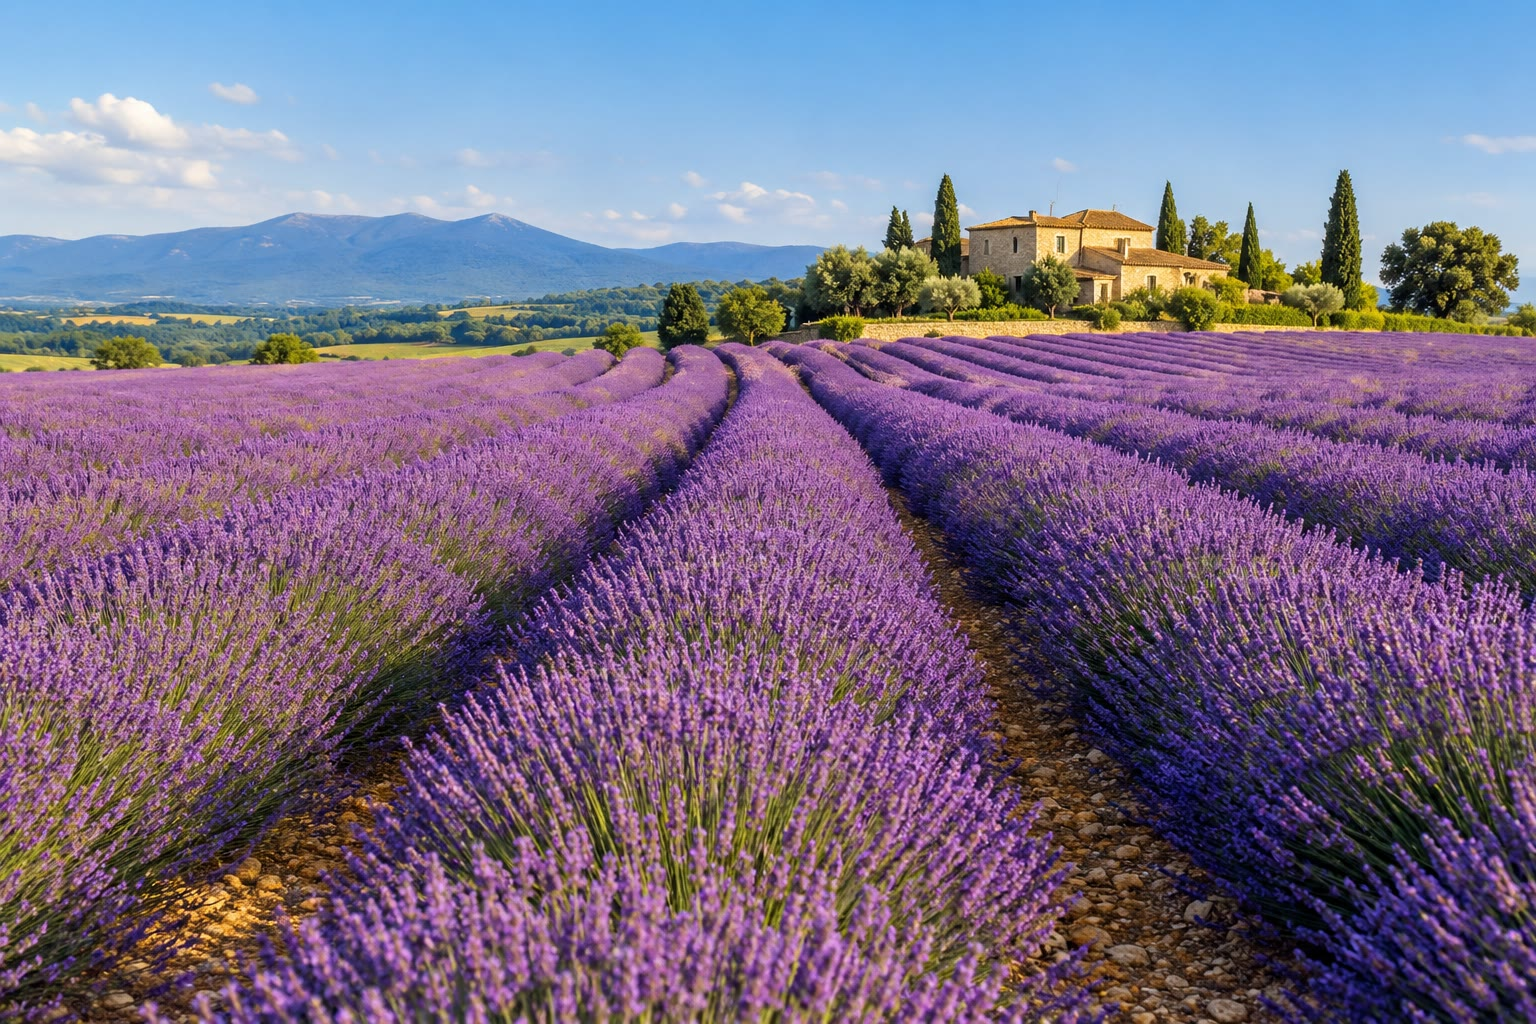
\includegraphics[width=0.55\linewidth]{images/book1/ai/g10-lavender-field.jpg}

{\small फूलों से भरा लैवेंडर का खेत: लैवेंडर सगंध तेल का
\omterm{def:g5:raw-materials-and-recycling:raw-material}{कच्चा माल}।}
\end{omfigure}

\section{अभ्यास}

\begin{exercise}[$\star$]\label{exo:g10:chemical-species:1}
प्राकृतिक या \omterm{def:g10:chemical-species:natural}{संश्लिष्ट स्पीशीज़}? वनीला की फली से मिला वैनिलिन; ऐस्पिरिन;
कॉफ़ी के बीजों से मिला कैफ़ीन; कारख़ाने में बना वैनिलिन।
\end{exercise}

\begin{exercise}[$\star$]\label{exo:g10:chemical-species:2}
संश्लिष्ट वैनिलिन और प्राकृतिक वैनिलिन का गलनांक एक ही क्यों
होता है?
\end{exercise}

\begin{exercise}[$\star$]\label{exo:g10:chemical-species:3}
एक TLC प्लेट पर \omterm{def:g6:solutions-and-solubility:solute}{विलायक} अग्र प्रारंभ-रेखा से \qty{6.0}{cm} ऊपर है
और एक धब्बा उससे \qty{2.4}{cm} ऊपर है। उसका $R_f$ निकालिए।
\end{exercise}

\begin{exercise}[$\star$]\label{exo:g10:chemical-species:4}
\omterm{def:g10:chemical-species:distillation}{आसवन} में संघनित्र की भूमिका बताइए, और बताइए कि ठंडा पानी उसके निचले सिरे से
क्यों प्रवेश करता है।
\end{exercise}

\begin{exercise}[$\star$]\label{exo:g10:chemical-species:5}
वे तीन शर्तें बताइए जो \omterm{def:g10:chemical-species:extraction}{निष्कर्षण} \omterm{def:g6:solutions-and-solubility:solute}{विलायक} को पूरी करनी चाहिए।
\end{exercise}

\begin{exercise}[$\star\star$]\label{exo:g10:chemical-species:6}
\omterm{def:g6:solutions-and-solubility:solute}{विलायकों} की सारणी की मदद से समझाइए कि आसुत से लिनालूल निकालने के लिए एथेनॉल
का उपयोग क्यों नहीं हो सकता, जबकि साइक्लोहेक्सेन का हो सकता है।
\end{exercise}

\begin{exercise}[$\star\star$]\label{exo:g10:chemical-species:7}
एक पृथक्कारी कीप में डाइक्लोरोमेथेन को पानी के साथ हिलाया जाता है। कौन-सी परत
ऊपर है? सारणी से पुष्टि कीजिए।
\end{exercise}

\begin{exercise}[$\star\star$]\label{exo:g10:chemical-species:8}
ऐस्पिरिन के नाम से बिकने वाला एक सफ़ेद चूर्ण \qty{126}{\celsius} पर पिघलना
शुरू होता है और \qty{132}{\celsius} पर पूरा पिघल जाता है। आप क्या निष्कर्ष निकाल सकते हैं?
\end{exercise}

\begin{exercise}[$\star\star$]\label{exo:g10:chemical-species:9}
इस अध्याय का TLC चित्र देखिए। लैवेंडर तेल में क्या है? कौन-सी
स्पीशीज़ ज़्यादा ऊपर चढ़ी?
\end{exercise}

\begin{exercise}[$\star\star$]\label{exo:g10:chemical-species:10}
प्रयोगशाला में लैवेंडर तेल पाने के चरणों को क्रम में लगाइए:
परतों को अलग करना; \omterm{def:g10:chemical-species:distillation}{जल-आसवन}; आसुत में साइक्लोहेक्सेन मिलाकर
हिलाना; साइक्लोहेक्सेन का \omterm{def:g3:separating-mixtures:evaporate}{वाष्पन}।
\end{exercise}

\begin{exercise}[$\star\star$]\label{exo:g10:chemical-species:11}
TLC प्लेट की प्रारंभ-रेखा पेंसिल से क्यों खींची जाती है और \omterm{def:g10:chemical-species:tlc}{निक्षालक} से ऊपर
क्यों रखी जाती है?
\end{exercise}

\begin{exercise}[$\star\star\star$]\label{exo:g10:chemical-species:12}
\omterm{def:g10:chemical-species:extraction}{निष्कर्षण} के बाद साइक्लोहेक्सेन को हल्का गरम करके हटा दिया जाता है, और तेल बच
जाता है। साइक्लोहेक्सेन और लिनालूल (\qty{198}{\celsius}) के क्वथनांकों की मदद से
समझाइए कि यह क्यों काम करता है।
\end{exercise}

\begin{exercise}[$\star\star\star$]\label{exo:g10:chemical-species:13}
किसी सुगंध का एक संश्लिष्ट नमूना TLC प्लेट पर \omterm{def:g10:chemical-species:natural}{प्राकृतिक स्पीशीज़} की ऊँचाई पर
एक धब्बा देता है, और सही ताप पर तीक्ष्णता से पिघलता है। आप कौन-से
दो निष्कर्ष निकाल सकते हैं?
\end{exercise}

\begin{exercise}[$\star\star\star$]\label{exo:g10:chemical-species:14}
उसी TLC में धब्बे A का $R_f = 0.40$ है और अग्र रेखा से \qty{5.5}{cm}
ऊपर है। धब्बा A कितनी ऊँचाई पर है? एक और स्पीशीज़ का
$R_f = 0.75$ है: वह धब्बे A से कितना ऊपर है?
\end{exercise}

\begin{exercise}[$\star\star\star$]\label{exo:g10:chemical-species:15}
\qty{1}{L} पानी में \qty{1.6}{g} लिनालूल घुल सकता है। \qty{200}{mL} पानी
वाले एक आसुत में \qty{0.20}{g} घुला हुआ लिनालूल है। क्या वह
संतृप्त है? वह कितना और घोल सकता है? इस पानी को फेंकने के बजाय साइक्लोहेक्सेन
से उसका \omterm{def:g10:chemical-species:extraction}{निष्कर्षण} करना क्यों उपयोगी है?
\end{exercise}

\clearpage % keeps the heading with its problem box (it was stranded at a page foot)
\section{समस्या: लैवेंडर की सुगंध}

\begin{problem}[{सप्ताहांत समस्या --- लैवेंडर के फूलों की एक टोकरी से सगंध तेल की
कुछ बूँदों तक, वर्णलेखन से जाँची गई}]
\label{pb:g10:chemical-species:1}
% ledger: rho:cyclohexane, bp:cyclohexane, rho:CH2Cl2, bp:linalool, ghs:cyclohexane
एक विद्यालय की प्रयोगशाला में \qty{100}{g} ताज़े लैवेंडर फूलों का पानी के साथ
\omterm{def:g10:chemical-species:distillation}{जल-आसवन} किया जाता है। धुँधले आसुत को पृथक्कारी कीप में
\qty{20}{mL} साइक्लोहेक्सेन के साथ हिलाया जाता है; साइक्लोहेक्सेन की परत
रखी जाती है, सुखाई जाती है, और साइक्लोहेक्सेन को हल्का गरम करके वाष्पित किया
जाता है। जो बचता है वह लैवेंडर सगंध तेल है। इस अध्याय की \omterm{def:g6:solutions-and-solubility:solute}{विलायकों} की
सारणी का उपयोग कीजिए।

\medskip
\noindent\textbf{भाग I --- \omterm{def:g10:chemical-species:distillation}{जल-आसवन}।}
\begin{enumerate}
  \item \omterm{def:g10:chemical-species:distillation}{जल-आसवन} में उबलते पानी की क्या भूमिका है?
  \item संघनित्र की क्या भूमिका है? ठंडा पानी उसमें कहाँ से प्रवेश
        करता है?
  \item आसुत में पानी पर तैरती एक पतली तैलीय परत दिखती है। क्या तेल पानी
        के साथ \omterm{def:g6:solutions-and-solubility:miscible}{मिश्रणीय} है? क्या वह पानी से कम घना है या अधिक?
  \item तेल पाने के लिए आसुत को सीधे-सीधे उँडेलकर अलग क्यों नहीं किया जाता?
\end{enumerate}

\medskip
\noindent\textbf{भाग II --- \omterm{def:g10:chemical-species:extraction}{निष्कर्षण}।}
\begin{enumerate}[resume]
  \item साइक्लोहेक्सेन इस \omterm{def:g10:chemical-species:extraction}{निष्कर्षण} के लिए उपयुक्त \omterm{def:g6:solutions-and-solubility:solute}{विलायक} क्यों है?
  \item क्या इसके बजाय एथेनॉल का उपयोग हो सकता था? समझाइए।
  \item हिलाने और ठहरने के बाद साइक्लोहेक्सेन की परत ऊपर है या
        नीचे? डाइक्लोरोमेथेन के साथ क्या होता?
  \item साइक्लोहेक्सेन के चित्रसंकेतों द्वारा अपेक्षित दो सावधानियाँ बताइए।
  \item लिनालूल, जो \qty{198}{\celsius} पर उबलता है, को खोए बिना
        साइक्लोहेक्सेन का \omterm{def:g3:separating-mixtures:evaporate}{वाष्पन} क्यों किया जा सकता है?
\end{enumerate}

\medskip
\noindent\textbf{भाग III --- वर्णलेखन।}
तेल, शुद्ध लिनालूल (L) और शुद्ध लिनालिल एथेनोएट (A) के धब्बे
एक TLC प्लेट पर लगाए जाते हैं। विकसित करने के बाद अग्र प्रारंभ-रेखा से
\qty{6.0}{cm} ऊपर है। तेल दो धब्बे देता है, \qty{2.4}{cm} पर और
\qty{4.5}{cm} पर; धब्बा L \qty{2.4}{cm} पर है, धब्बा A \qty{4.5}{cm} पर।
\begin{enumerate}[resume]
  \item लिनालूल और लिनालिल एथेनोएट के $R_f$ निकालिए।
  \item जहाँ तक यह प्लेट दिखाती है, तेल में क्या है?
  \item क्या लैवेंडर तेल एक \omterm{def:g6:pure-substances-and-mixtures:pure-substance}{शुद्ध पदार्थ} है?
  \item संदर्भों के धब्बे तेल वाली प्लेट पर ही क्यों लगाए गए?
  \item एक संश्लिष्ट लिनालूल का धब्बा उन्हीं परिस्थितियों में चलाई गई दूसरी प्लेट
        पर लगाया जाता है: उसका $R_f = 0.40$ है। क्या निष्कर्ष निकाला जा सकता है?
\end{enumerate}

\medskip
\noindent\textbf{भाग IV --- कितना तेल?}
मिला हुआ तेल \qty{1.0}{mL} भरता है; इस तेल के \qty{1}{mL} का भार
\qty{0.90}{g} है।
\begin{enumerate}[resume]
  \item कितने द्रव्यमान का तेल मिला?
  \item यह फूलों के द्रव्यमान का कितना प्रतिशत है?
  \item \qty{100}{g} तेल के लिए कितने द्रव्यमान के फूल चाहिए होंगे?
  \item तेल को ``प्राकृतिक'' कहा जाता है। यह किस अर्थ में सच है? क्या
        उसका लिनालूल संश्लिष्ट लिनालूल से अलग है?
  \item \qty{100}{g} फूलों से मिले सगंध तेल का द्रव्यमान
        बताइए।
\end{enumerate}
\end{problem}
